\documentclass[10pt, A4]{article}
\usepackage[left=1.2in, right=1.2in, top=1.2in, bottom=1.5in]{geometry}
\usepackage{fancyhdr}
\usepackage{xcolor}
\usepackage{floatrow}
\usepackage{amsmath}
\definecolor{newcol}{RGB}{150, 10, 15}
\usepackage{amsthm}
\usepackage{amssymb}
\usepackage{esint}
\usepackage{listings}
\usepackage{graphicx}
\usepackage{multirow}
\usepackage{mdframed}
\usepackage{multicol}
% \usepackage{achemso}
\usepackage[linesnumbered,ruled, lined, vlined]{algorithm2e}
\usepackage{lineno}
\usepackage{enumerate}
\usepackage[document]{ragged2e}
\usepackage{hyperref}
\newcommand*{\daggerfootnote}[1]{%
	\setcounter{daggerfootnote}{\value{footnote}}%
	\renewcommand*{\thefootnote}{\fnsymbol{footnote}}%
	\footnote[2]{#1}%
	\setcounter{footnote}{\value{daggerfootnote}}%
	\renewcommand*{\thefootnote}{\arabic{footnote}}%
}
\newcounter{code}[section]
\lstnewenvironment{code}[2]{
	\refstepcounter{code}
	\center{\large{\textbf{Listing \thecode: #1}}}
	\vspace{-0.8em}
	\textbf{\normalsize{\center{#2}}}
	\lstset{language=#1,
		numbers=left,
		escapeinside={\%*}{*)},
		numberstyle=\tiny\color{gray},
		breaklines=true,
		stringstyle=\color{violet},
		keywordstyle=\color{blue}\bfseries,
		identifierstyle=\color{black},
		commentstyle=\color{green!30!black},
		moredelim=*[s][\color{newcol}]{\$}{\$}
	}
}{}
\hypersetup{colorlinks=false, linkcolor=black,linkbordercolor=red,pdfborder={0,0,1}}
\pagestyle{fancy}
\fancyhf{}
\lhead{190050032-19D070024}
\rhead{Software Systems Laboratory}
\cfoot{Page \thepage}
\renewcommand{\footrulewidth}{1 pt}
\AtBeginDocument{\hypersetup{pdfborderstyle={/S/S/W 1}}}
\begin{document}
	\title{\LaTeX{} Starter Pack}
	\author{190050032-19D070024}
	\date{August 30, 2020}
	\maketitle
	\tableofcontents
	\thispagestyle{empty}
	\newpage
	\pagenumbering{arabic}
	\section{Introduction}
	\label{sec:Intro}
	\LaTeX{} (most popularly pronounced lay-tech; sometimes laa-tech) is an incredibly efficient office
	tool to typeset professional looking technical documents and reports. You will certainly find it
	useful to write assignments, format your resume, and more generally, to make everything you do
	look cooler.\vspace{0.5em}\\
	\LaTeX{}, like HTML, is a \textbf{markup language}. It’s part of \TeX{} typesetting system created by
	the immortal Donald Knuth. The presentation of the content depends on the properties of the
	tags it is wrapped in. For more involved typesetting purposes, this gives it a clear edge over
	mainstream word processors like {\color{blue}MS-Word}: in Word,\textit{what you see is what you get}, and getting
	what you want can be insanely tough.
	\vspace{0.5em}\\
	Here's how it works: you write your markup commands in the source file, which has a \texttt{.tex}
	extension. You need “software”, or formally, a \ distribution, to actually typeset them into a
	format suitable for \TeX{} distribution, which is generally a pdf. The most popular distribution to install
	on your machine is TeX Live; MikTeX is an alternative. You could also work online with Overleaf
	- no installations, and a ridiculously straightforward workflow. This is ideal for smaller projects.
	Weigh your options \href{https://www.latex-project.org/get/}{here}. Yes, a hyperlink!\vspace{0.5em}\\
	\LaTeX{} allows us to write complex mathematical equations without much fuss; its environments
	save us the hassle of organising large documents manually; with \LaTeX{} we can showcase code and
	render almost any scientific illustration. \LaTeX{} is paradise for anyone who works in STEM. Once
	you have experience, you can typeset assignments, papers, articles and theses with unprecedented
	ease.\vspace{0.5em}\\
	{In this assignment, we will explore and demonstrate some features that often prove themselves
		useful for several purposes}.\vspace{0.5em}\\
	{\large In this introductory section, we have also seen how we can format text. For instance,
		we can make text bold, italicized, colour it, or manipulate its size, and even toggle
		between alignments!}\\
		\vspace{2em}
	
	\hspace{11cm}{\color{newcol}\Large{\textsc{Carpe Diem!}}}\\
	
	\begin{figure}[H]
		\centering
		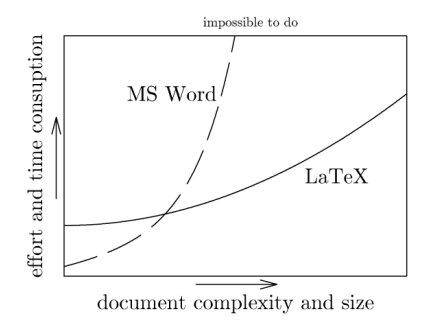
\includegraphics[width=0.6\linewidth]{ease-graph.png}
		\caption{This graph by Marko Pinteric is spot on.}
	\end{figure}
	
%%%%%%%%%%%%%%%%%%%%%%%%%%%%%%%%%%%%
% page 2
%%%%%%%%%%%%%%%%%%%%%%%%%%%%%%%%%%%%

\section{Basic Document Formatting}
\label{sec:basic}
In STEM, brevity is highly valued. You want to put forth your arguments as crisply as possible.
Of course, sometimes a rather long clarification may be in order\footnote{ Footnotes are a classy way to do that. Making footnotes is fairly simple in \LaTeX.}, however, it is better to stick
to the central theme and not disrupt the flow. In order to make your point, lists are often the
cleanest option.
\subsection*{Features we demonstrate}
\begin{itemize}
	\item Making a title and table of contents
	\vspace{-0.3em}
	\item Organising the document into sections
	\vspace{-0.3em}
	\item Setting up the page layout
	\vspace{-0.3em}
	\item Designing our custom header and footer
	\vspace{-0.3em}
	\item Formatting text
	\vspace{-0.3em}
	\item Making (nested) lists
	\vspace{-0.3em}
	\begin{enumerate}
		\item itemize
		\vspace{-0.3em}
		\item enumerate
		\vspace{-0.3em}
		\item description
		\vspace{-0.3em}
	\end{enumerate}
	\item Footnotes
	\vspace{-0.3em}
	\item Typesetting mathematics
	\vspace{-0.3em}
	\item Theorem and Proof environments
	\vspace{-0.3em}
	\item Hyperlinks and cross references within the document
	\vspace{-0.3em}
	\item Custom environments
	\vspace{-0.3em}
	\item Algorithms and code
	\vspace{-0.3em}
	\item Inserting images
	\vspace{-0.3em}
	\item Drawing tables
	\vspace{-0.3em}
	\item Citations\daggerfootnote{using BibTeX, which automatically takes care of the bibliography formatting}
\end{itemize}
\vspace{-.4em}
In order to make your lists appear more concise, you can specify the \texttt{itemsep} parameter as an
optional argument to the environment. You will need the \texttt{enumitem} package for that.\vspace{0.5em}\\
Descriptive lists are sometimes handy:
\vspace{-0.5em}
\begin{description}
	\item [CS 207] Discrete Structures
	\vspace{-0.8em}
	\item [CS 213] Data Structures and Algorithms
	\vspace{-0.8em}
	\item [CS 215] Data Analysis and Interpretation
	\vspace{-0.8em}
	\item [CS 251] Software Systems Lab
	\vspace{-0.8em}
	\item [CS 293] Data Structures and Algorithms Lab
	\vspace{-0.5em}
\end{description}
\subsection*{The Page Layout}
\vspace{-.5em}
The paper size for this document is A4. The left and right margins are 1.2 inches each; the lower
margin is 1.5 inches. The geometry package is very convenient to set up and manipulate these
dimensions.
\vspace{1.5em}

%%%%%%%%%%%%%%%%%%%%%%%%%%%%%%%%%%%%
% page 3
%%%%%%%%%%%%%%%%%%%%%%%%%%%%%%%%%%%%

\section{Mathematics}
\label{math}

Make sure you have imported the \texttt{amsmath}, \texttt{amsthm}, \texttt{amssymb} and \texttt{esint} packages, in that order.
Have a look at the tutorial to understand how they work, and what they do. In particular, the
\texttt{amsthm} package makes defining ordered theorem-like environments very convenient.\vspace{0.5em}\\

\textbf{Theorem 1}\label{theorem1} (Markov’s Inequality). \textit{If $\text{X}$ is a non-negative random variable and a $\ge$ 0 then}
$$P(X \ge a) \le \frac{E(X)}{a}$$

\textbf{Corollary 2}\label{corollary2} (Chebyshev’s Inequality).\textit{Let $\text{X}$ be an integrable random variable with finite expected
	value $\mu$ and finite variance  $\sigma^2$ $\ne$ 0. Then for any $k \in R$, k \textgreater 0,}
$$P( \lvert X-\mu\rvert \ge k\sigma) \le \frac{1}{k^2}$$

\textit{Proof}. Let the random variable $Y :=(X- \mu)^2$.Observe that Y is a non-negative random variable;
and from the definition of variance, $E(Y ) = \sigma^2$ , which is positive from the premise. Hence, we
can appeal to Theorem \hyperref[theorem1]{1}.
$$P(Y \ge k^2 \sigma^2) \le \frac{\sigma^2}{k^2\sigma^2} = \frac{1}{k^2}$$

However, $P (Y \ge k^2\sigma^2 ) = P (\lvert X-\mu \rvert \ge k\sigma)$ and we are done.\\

\vspace{0.8em}
Consider a plane $z = ax + by + c$. Usually, three poin ts on the plane are sufficient to determine
the parameters $a, b, c$; however, we’re given a data set of several points: $x$ and $y$ coordinates are
known perfectly, but the $z$ coordinates are corrupted by a Gaussian noise $\mathcal{N}(0, 1)$. Here’s how we
solve for the maximum likelihood estimates of the parameters:

%-----------------matrix
\begin{equation}
	\label{equation1}
\begin{bmatrix}
	\sum_{i} x_{i}^2 & \sum_{i} x_{i}y_{i} & \sum_{i} x_{i}\\
	\sum_{i} x_{i}y_{i} & \sum_{i} y_{i}^2 & \sum_{i} y_{i}\\
	\sum_{i} x_{i} & \sum_{i} y_{i} & \sum_{i} 1\\ 
\end{bmatrix}
\begin{bmatrix}
	\hat a\\
	\hat b\\
	\hat c\\
\end{bmatrix}
=
\begin{bmatrix}
	\sum_{i} x_{i}z_{i}\\
	\sum_{i} y_{i}z_{i}\\
	\sum_{i} z_{i}\\
\end{bmatrix}
\end{equation}

The above equation (we can also refer to it as equation \hyperref[equation1]{1}  as we created a label) is obtained by
setting the partial derivatives of the log-likelihood to 0, eg. $\partial L/\partial a = 0$ etc.
\vspace{0.5em}
Observe that we also cross referenced Theorem \hyperref[theorem1]{1} in the proof of Corollary \hyperref[corollary2]{2}. And here we just
did it again. This is how we use labels in tandem with the \texttt{hyperref} package.\\
\vspace{0.5em}
\textbf{Theorem 3} (De Morgan’s Law). $\neg(a \lor b) \iff \neg a \land \neg b$. Alternately, in the context of sets, we
have $\overline{A \cup B} =\overline{A} \cap \overline{B}$.\\
\vspace{0.5em}
$Remark$. This is closely related to the following rule in first order propositional logic: $\neg(\exists x.p(x))\iff
\forall x.\neg p(x)$\\
\vspace{0.5em}
We almost always want to cite sources for claims we make, because when you publish, it’s pointless
to keep reinventing the wheel. For instance, the Kronecker’s Theorem on simultaneous Diophantine
approximations is a standard but powerful result, it makes sense to refer the reader to [\cite{bourbaki1966general}, Chap.
7, Sec. 1.3, Prop. 7] for a statement and proof. This source is a book. Make sure you enter the
relevant information in the appropriate fields in the BibTeX entry.\\
\vspace{0.5em}
In Computer Science, most citations are journal or conference papers. A discussion on algebraic
numbers is incomplete without citing the Mignotte separation bounds, given in a modestly titled
conference paper \cite{mignotte1982some}. We can even cite multiple sources with a single command \cite{bell2007positivity,renegar1992computational}. These are
journal articles. If possible, it’s best to also specify the volume and page numbers. Your aim
should be to point the reader to what you’re quoting as unambiguously as possible.\\
	

%%%%%%%%%%%%%%%%%%%%%%%%%%%%%%%%%%%%
% page 4
%%%%%%%%%%%%%%%%%%%%%%%%%%%%%%%%%%%%

\section{Computer Science}
\subsection{Algorithms}
We have used the \texttt{algorithm2e} package.

\begin{algorithm}
	\SetAlgoLined
	\DontPrintSemicolon 
	\caption{Dijkstra's algorithm}
	\KwData{Graph, source}
	\KwResult{Distances of each vertex from the source and starting edges of the shortest paths}
	create priority queue $Q$ of vertices of Graph //min-heap\;
	\ForEach{vertex v in Graph}{
		$dist[v] \gets \infty$\;
		$prev[v] \gets$ UNDEFINED\;
		add $v$ to $Q$\;
	}
	$dist[source] \gets 0$\;
	\While{{$Q$ is not empty}}{
		$u \gets Q.extract()$\;
		\ForEach{{neighbour $v \in Q$ of  u}}{
			$alt \gets dist[u] + length(u,v)$\;
			\If{$alt < dist[v]$}{
				$dist[v] \gets alt$\;
				$prev[v] \gets u$\;
			}
		}
	}
	return $dist[],prev[]$\;	
\end{algorithm}

\subsection{Environments \& Code}

\label{thelistingpackage}
\begin{code}{[LaTeX]TeX}{The Listings Package}
\begin{lstlisting}
%Your code goes here.
		
%This is usually how you present code in \LaTeX, without worrying about accidentally invoking a macro.Yes, the text is displayed verbatim .
\end{lstlisting}
\label{trickq}
\end{code}
\vspace{0.8cm}
For our document, however, we noticed that na\"{i}ve methods don’t work, and defined a custom
%naive to be rewritten
environment with \texttt{\textbackslash lstnewenvironment}. This takes care of title formatting and vertical spacing
too! Our environment has a counter associated with it, and takes the language and title as
arguments. Other code formatting options are specified with \texttt{\textbackslash lstset\{...\}}. You might want to
have a look at the tutorial!\\
\newpage
\label{algorithmboilerplate}
\begin{code}{[LaTeX]TeX}{Algorithm Boilerplate}\label{listing2}
\documentclass{article}
%...
\usepackage [linesnumbered,ruled,vlined] {algorithm2e}
%. . .
\begin {document}
%. . .
\begin {algorithm} [h]
\caption {...}
\SetAlgoLined
\DontPrintSemicolon
\KwData{...}
\KwResult{...}
Statement \;
%Let magic happen here
$1+1=2$ \;
\end{algorithm}
%...
\end{document}
\end{code}
\vspace{0.5cm}
\begin{code}{Bash}{Another Language}
#some keywords
for echo cat case if esac elif fi awk sed pwd while do
sudo apt-get update sleep
\end{code}
\vspace{0.5cm}
\begin{code}{Python}{Keywords,comments,strings}
from numpy import *
#insanely powerful library
print("Hello Everyone!")
\end{code}
\vspace{1cm}
%lstset and lstnewenvironment not set
The advantage of defining ordered environments like this is that you can refer to this pretty easily if
you’ve left a label properly. If you want to shift them around, the counter and the cross references
will do the adjustment automatically. Of the above, Listing \hyperref[thelistingpackage]{1} is a fiendish trick question, and
Listing \hyperref[algorithmboilerplate]{2} is rather benevolent.
\newpage
%%%%%%%%%%%%%%%%%%%%%%
%page 6
%%%%%%%%%%%%%%%%%%%%%%
\vspace{-0.5em}
\section{Utilities}
\subsection{Images}

You’ll sometimes find the need to include images in your report. Ideally, the images should
enhance the document. But yeah, you’re probably going to use this technique for a rather dirty
life hack. If a Prof insists on a \LaTeX{} report, you’re just going to dump a photo of your exquisite
handwriting to save time, aren’t you? \textit{Exploit this loophole at your own risk. The original author
	of this assignment can neither confirm nor deny his endorsement of the jugaad.}

\begin{figure}[H]
	\centering
	\begin{floatrow}
		\ffigbox[0.4\textwidth]{\caption{Aristotle: The first formal
				logician.} } {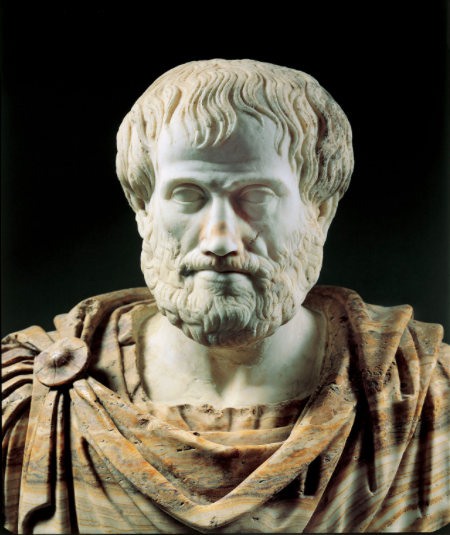
\includegraphics[width=0.4\textwidth]{aristotle.png}}
		
		\ffigbox[0.4\textwidth]{\caption{Saul Kripke: we’ve come a long way
				since then.} } {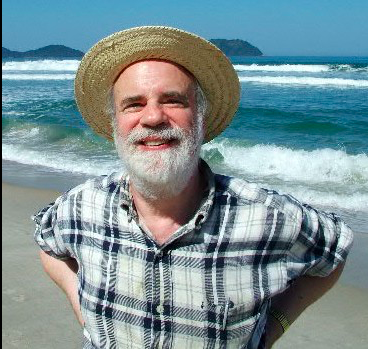
\includegraphics[width =0.5\textwidth]{kripke.png}}
	\end{floatrow}
\end{figure}

\begin{raggedright}
\href{https://www.britannica.com/biography/Aristotle#/media/1/34560/76426}{Aristotle image source}\\
\end{raggedright}
\href{https://commons.wikimedia.org/w/index.php?curid=5763037}{Saul Kripke image source}\\
Make sure you follow these links, so you know where the hyperlinks lead to when you typeset it
yourself.
\vspace{-0.5em}
\subsection{Tables}
\vspace{-0.5em}
\begin{table}[H]
	\begin{tabular}{c|l}
		\hline
		\textbf{Complexity} & \textbf{Examples} \\
		\hline
		{$\mathcal{O}(1)$} & Computing \\
		\hline 
		\multirow{2}{*}{$\mathcal{O}(log(n))$} & Binary Search \\
		& Insertion \& Removal from a min-heap\\
		\hline
		\multirow{2}{*}{$\mathcal{O}(nlog(n))$} & Merge Sort \\
		& Fast Fourier Transform\\
		\hline
		\multirow{2}{*}{$n^2$} & Bubble Sort \\
		& First attempt at a problem which has a linear time solution\\
		\hline
		$2^{\mathcal{O}(log(n))}$ & AKS Primality Test\\
	\hline
	\multicolumn{2}{c}{You might want to define a macro to write this notation conveniently}\\
	\hline 
\end{tabular}
\caption{Some common time complexities}
\end{table}
This table uses \texttt{multirow} as well as \texttt{multicolumn}. Replicate it as well as you can.\\
We have used the fairly popular \texttt{plainurl} style.

\bibliographystyle{plain}
\bibliography{my_starter_pack}

\end{document}